\documentclass[journal]{IEEEtran}
\usepackage{amsmath}
\usepackage{cite}
\usepackage{graphicx}

\title{Against the Correlation Length as Minimum Secure Distance in Link Signature Keying}
\author{K.~C.~Kerby-Patel,~\IEEEmembership{Senior Member, IEEE}
\thanks{K.~C.~Kerby-Patel is with the Engineering Department, University of Massachusetts Boston, Boston, MA 02125 USA e-mail: kc.kerby-patel@umb.edu}}%
\begin{document}
\maketitle
\begin{abstract}
An argument is presented against the use of the channel correlation function to derive the minimum secure distance in link signature keying.  It is observed that mutual information between channel observations at two locations may persist over distances greater than the correlation length, and thus an eavesdropper could obtain some information about the legitimate nodes' channel measurement.  Example simulations are presented to illustrate situations in which the correlation function has a much narrower peak than the mutual information.
\end{abstract}
\begin{IEEEkeywords}
link signature, key generation, physical layer security, mutual information, correlation
\end{IEEEkeywords}
\IEEEpeerreviewmaketitle

\section{Introduction}
Link signature keying (LSK) uses the inherent reciprocity and location dependence of the wireless channel to generate symmetric encryption keys for a pair of nodes in a wireless network.  The channel transfer function serves as a common source of information that is used as the random number seed for key generation.  It has been suggested that LSK may be information-theoretically secure \cite{ye2010}, which would make it an attractive alternative to computational key exchange techniques.
	
Since LSK depends on the physical parameters of the channel, the security metric for this technique is a minimum secure distance (MSD).  An eavesdropper separated from both of the legitimate nodes by at least the MSD is unable to estimate the legitimate nodes' key because it has insufficient knowledge of the channel transfer function between them.  Common practice is to use the channel correlation length as the MSD, which is often further approximated as a half wavelength \cite{azimisadjadi2007, bloch2008, mathur2008, ye2010}. 

He et al. \cite{he2013} have pointed out that the correlation length of Rayleigh fading channels is a half wavelength, but other channels may have much longer correlation lengths.  In this communication, we further observe that mutual information is likely to persist over distances greater than the correlation length because of the oscillatory nature of the channel transfer function and its autocorrelation.  We present a Monte Carlo simulation of an example channel in which this is the case.  Based on this evidence, we argue that a more conservative means of estimating the MSD is necessary.

\section{Argument}
%Add a figure here, introduce Alice, Bob, and Eve
Consider a wireless channel with two legitimate nodes, Alice and Bob, and an eavesdropper Eve (Figure \ref{scenario}).  Eve is permitted to take samples of the channel transfer function at multiple locations; later we will consider the particular situation where these samples are constrained to lie along a line toward Bob as pictured.
\begin{figure}
\begin{center}
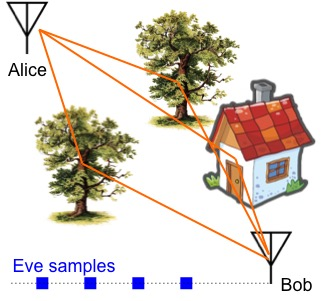
\includegraphics[width=2.75in]{scenarioEve}
\caption{Notional link signature keying scenario with legitimate nodes Alice and Bob, and eavesdropper Eve.}\label{scenario}
\end{center}
\end{figure}

The metric of information theoretic security, and in general of an eavesdropper's ability to estimate the legitimate nodes' channel, is the mutual information between Eve's observations of the Alice-to-Eve channel transfer function $\hat{h_{AE}}=h_{AE}+n_E$ and Bob's observations of the legitimate channel $\hat{h_{AB}}=h_{AB}+n_B$. The commonly accepted use of the correlation length as the MSD implicitly uses the correlation function as a proxy for the mutual information function.  If the two channel transfer functions are jointly Gaussian random variables, the mutual information $I$ is in fact a monotonic function of the statistical correlation $\rho$, and such an analogy is appropriate \cite{cover2006-jgvars}:
\begin{equation}\label{JGMI}
I(h_{AE}+n_E;h_{AB}+n_B) = -\frac{1}{2}\log (1-\rho^2)
\end{equation}
However, if the channel observations are not jointly Gaussian, (\ref{JGMI}) is merely a lower bound for the mutual information between Bob's and Eve's channel observations.  In general, environmental channel parameters such as the angle of a particular scattering path have been observed to persist over distances greater than the correlation length \cite{jakes1974, duel-hallen2007}.  
%Here, I might need to articulate the step in the argument where I say that since h is a deterministic function of the vars, and the vars persist, the MSD could also persist (depending on the operation performed by h) - data processing inequality.
This indicates that in realistic channels the mutual information may also persist longer than the correlation length. In such a situation, the mutual information is indeed greater than that indicated by (\ref{JGMI}).  Thus, estimates of the MSD based on the correlation length are in general optimistic.



Physically, the channel is a deterministic function of a set of environmental parameters $\vec{\theta}$ that describe nearby scatterers - for instance, the scatterers' positions and the amplitudes and phases of reflected waves relative to some transmitter.  The environmental parameters at an arbitrary pair of observer positions can be considered to have a position-dependent joint probability density function.  Intuitively, the two sets of channel parameters must approach equality (complete dependence) when the distance between observation points approaches zero, and complete independence when the distance approaches infinity.  
%implicitly, chan params are a random process (function of observer position rather than t, assuming channel is not time-varying)
If we make no other assumptions about this probability density function, then the mutual information between Eve's and Bob's channel transfer functions $\hat{h}_{AE}$ and $\hat{h}_{AB}$ is trivially bounded by $I(\vec{\theta}_E;\vec{\theta}_B)$ via the data processing inequality; in the case of zero separation between observation points this becomes $H(\vec{\theta})$.



%do we actually need the equations here?  This stuff is pretty basic probability and info theory
%The channel transfer functions $h_{AE}$ and $h_{AB}$ are not one-to-one functions of the channel parameters, so we cannot compute their probability distribution functions directly.  However, it is always possible to find a joint cumulative distribution function $F$ for the real and imaginary parts of $h_{AE} = g_E(\vec{\theta}_E)=R_E+jX_E$; and $h_{AB}=g_B(\vec{\theta}_B)=R_B+jX_B$, based on the joint probability density function of $\vec{\theta}_E$ and $\vec{\theta}_B$.  
%\begin{multline}
%F(r_E,x_E,r_B,x_B) = \\Pr\{R_E \leq r_E, X_E \leq x_E, R_B \leq r_B, X_B \leq x_B \}
%\end{multline}
%The joint probability density function $p$ for the components of the channel transfer functions is given by
%\begin{equation}
%p(r_E,x_E,r_B, x_B) = \frac{\partial^4 F(r_E,x_E,r_B, x_B)}{\partial r_E \partial x_E \partial r_B \partial x_B}
%\end{equation}
%The mutual information between the main channel and eavesdropper channel can then be computed from the probability density function:
%\begin{multline}
%I(h_{AE}; h_{AB}) = I(R_E, X_E; R_B, X_B) = \\
% H(R_E)+H(X_E|R_E) -H(R_E|R_B,X_B) \\- H(X_E|R_E,R_B,X_B)
%\end{multline}


%Do I want this section?
%\section{Estimation Theoretic Formulation}
%\begin{itemize}
%\item Mutual information may be difficult to calculate in practice; the probability distribution of scatterers might be poorly defined
%\item Instead propose an analysis of eavesdropper capabilities based on estimation theory for the case that $\vec{\theta}$ is approximately constant within the observation window (corresponds to scatterers in the far field) \cite{kckpVTC2015}
%\item we get a minimum value for the variance of an unbiased estimate
%\item assume the joint probability distribution that maximizes mutual info for given means and variances
%\end{itemize}

\section{Example Scenario}
In this section we present a simulated example in which the mutual information between spatially separated channel observations is shown to decrease more slowly than the correlation between observations.  In this example, we estimate the mutual information between two spatially separated channel observations by a histogram method. While this technique is not a particularly accurate method of estimating the mutual information between \emph{continuous} variables, it is a realistic model of the \emph{discretized amplitude and phase} that would be involved in practical LSK implementations.  The similarity to real-life application justifies the use of this simplistic estimation technique.  The example scenario will examine the effect of various discretization decisions.

We use a sum-of-sinusoids channel model in which the $n$th scattering path's complex amplitude $\alpha_n(r)$ and direction of arrival $\phi_n(r)$ are spatially dependent (rather than time-dependent) random processes.  The scattering path amplitude $\alpha_n(r)$ is assumed to be a zero-mean complex Gaussian process.  The direction of arrival $\phi_n(r)$ is assumed to be a real Gaussian process with mean $\mu_n$ which is uniformly distributed in $[0, 2\pi)$ and fixed for each path in each channel realization.  Both parameters are assumed to have a covariance function that enforces the spatial dependence requirements described in the earlier section.  Thus, the value of a particular channel transfer function realization at an observation point $r$ is
\begin{equation}
h(r) = \sum_{n=1}^N \alpha_n(r) e^{-jkr\sin(\phi_n(r))}
\end{equation}
%if I leave it this way and don't make mu vary randomly with position, mutual information will not go to zero with distance.
%cite Duel-Hallen or others for examples of reasonable choices for characteristic length.
%In time-varying channels the parameters' random processes may also be time-dependent.
%We are not aware of any previous work that describes the spatial dependence of channel parameters in detail.
%*Hopefully* example will show that choice of correlation function and/or probability distribution of the parameters doesn't have a strong effect on the issue at hand, which is the speed at which correlation falls off as compared to mutual information.

For each distance between pairs of channel observations, an ensemble of many channel realizations is used to estimate both the mutual information and the correlation function.  Thus, the correlation function used here is a true ensemble average of $h(r)h(r-R)$ and not the spatial average that is commonly used to approximate it.  %As such, it does not imply any assumption of stationarity.


\section{Conclusion}
%MSD based on correlation function is probably optimistic.  Need a more conservative MSD.
%estimation theory approach (like in \cite{kckpVTC2015}) 
\bibliographystyle{IEEEtran}
\bibliography{PL-Library}{}
\end{document}